\documentclass[12pt]{article}
%Gummi|065|=)
\usepackage{amsmath, amsfonts, amssymb}
\usepackage[margin=0.5in]{geometry}
\usepackage{xcolor}
\usepackage{graphicx}
\usepackage{ifthen}

\usepackage{pifont}
\usepackage{amsmath}

\newcommand{\off}[1]{}
\DeclareMathSizes{20}{30}{20}{18}

\newcommand{\two }{\sqrt[3]{2}}
\newcommand{\four}{\sqrt[3]{4}}
\newcommand{\red}{\begin{tikz}[scale=0.25]
\draw[fill=red, color=red] (0,0)--(1,0)--(1,1)--(0,1)--cycle;\end{tikz}}
\newcommand{\blue}{\begin{tikz}[scale=0.25]
\draw[fill=blue, color=blue] (0,0)--(1,0)--(1,1)--(0,1)--cycle;\end{tikz}}
\newcommand{\green}{\begin{tikz}[scale=0.25]
\draw[fill=green, color=green] (0,0)--(1,0)--(1,1)--(0,1)--cycle;\end{tikz}}

\newcommand{\sq}[3]{\draw[#3] (#1,#2)--(#1+1,#2)--(#1+1,#2+1)--(#1,#2+1)--cycle;}
\newcommand{\linebrk}{----------------------------------------------------------------------------------------------------------------------------------}


\usepackage{tikz}

\newcommand{\susy}{{\bf Q}}
\newcommand{\RV}{{\text{R}_\text{V}}}

\title{Tutorial : Quadratic Reciprocity}
\date{}
\begin{document}

\fontfamily{qag}\selectfont \fontsize{12.5}{15}\selectfont

\maketitle

\noindent Reciprocity Theorems: why do they happen?  why are they important?  Every time I see a proof of quadratic reciprocity it's usually at the end of a textbook just to show off all the ``concepts" we have learned.  For me, the argument's tell me it's true but if we are trying to solve the equiation:
$$ x^2 \equiv p \pmod q $$
it doesn't explain why $p \leftrightarrow q$ should be possible, why these numbers should be on equal footing.  And if we look at other ``reciprocity theorems"  can their proofs be told in ``elementary" language i.e. with numbers! \\ \\
These days I find the Legendre symbol misleading.  Let's try another way:
$$ \Big[ x^2 \equiv p \pmod q \Big] \leftrightarrow \Big[ x^2 \equiv q \pmod p \Big]  $$
except this is not true when but $p = 4k+3$ and $q = 4k + 3$ then we have the opposite
$$ \Big[ x^2 \equiv p \pmod q \Big] \leftrightarrow \Big[ x^2 \not\equiv q \pmod p \Big]  $$
How is this applied in the real world?  I think that's an open question.  All I can say is that the concept of the integers $\mathbb{Z}$ becomes are scaffolding for understanding a chaotic world, that really has no intrinsic concept of number.\footnote{Why is there no \textbf{dynamical systems}  proof of Quadratic Reciprocity?  We will not discuss {\color{black!10!white}cryptrography} in any way, but maywe we could discuss \textbf{coding}  or \textbf{information theory}.  Just, number theory is to as ``applied" as one would like.  Philosophically it's about abstracting away from the real world something extremely pure.} \\ \\
Can you come up with a better concept than $\mathbf{0}$ or better than $\mathbb{Z}$?  No. \\ \\ \\ \\
Usually the justification is that Quadratic Reciprocity is connect to other branches of mathematics.  Let's try:
$$ \big[ \text{fermat's little theorem(s)} \big]
\to \big[ \text{QR} \big]
\to \big[ \text{three squares} \big] 
\to \big[ \text{Banach-Tarski paradox} \big]$$


\newpage

\noindent \textbf{A} Wikipedia has a separate page for \text{proofs} of Quadratic Reciprocity.  Let's try the willy-nilly Eisenstein proof, which I despise. \\ \\
Theorem {\color{orange!75!green}\textbf{98}} of Hardy's ``Introduction to the Theory of Numbers" states:
$$ \left(\frac{p}{q}\right) \left(\frac{q}{p}\right) = (-1)^{\frac{p-1}{2} \frac{q-1}{2}} $$
for any two odd primes $p$ and $q$. And {\color{orange!75!green}\textbf{99}}={\color{orange!75!green!50!white}\textbf{98}} splitting into the two cases:
$$\begin{array}{cccl}
x^2  \equiv q \pmod p & \leftrightarrow  & x^2  \not \equiv  p \pmod q &
\text{if }  p = 4k+3, q = 4k+3 \\ \\
x^2  \equiv q \pmod p & \leftrightarrow  & x^2  \equiv  p \pmod q &  
\text{otherwise}  \\
\end{array}$$
And there is theorem {\color{orange!75!green}\textbf{100}} which is a lemma about lattice point counting:
$$ \sum_{s = 1}^{\frac{p-1}{2}}  \left[ \frac{s\,q}{p} \right]
+ \sum_{s = 1}^{\frac{q-1}{2}}  \left[ \frac{s\,p}{q} \right] = \frac{p-1}{2} \cdot \frac{q-1}{2}$$

% http://latex.org/know-how/latex/51-latex-math-science/513-tikz-math
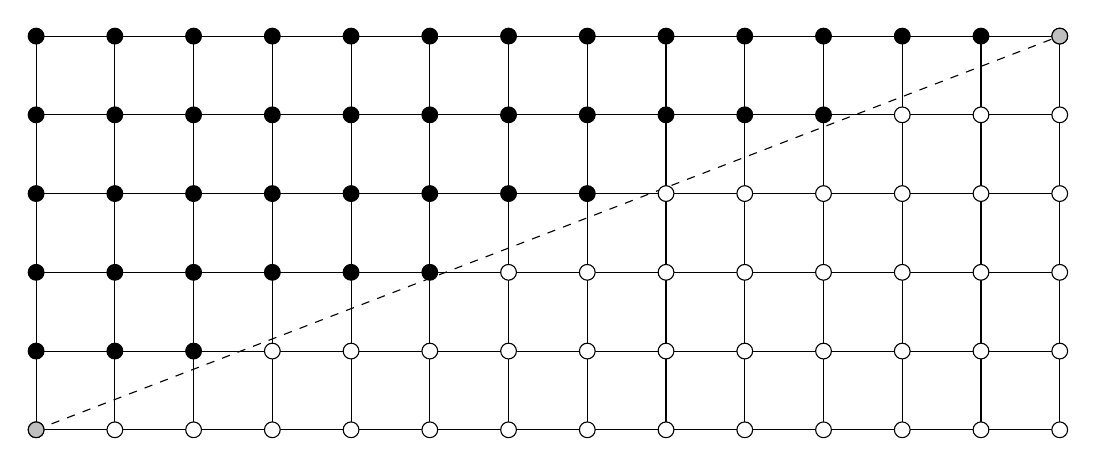
\begin{tikzpicture}

    \draw[dashed] (0,0)--(13,5);

    \foreach \a in {0,...,5}{
        \draw (0,\a)--(13,\a);
    }
    \foreach \a in {0,...,13}{
        \draw (\a,0)--(\a,5);
    }

    \foreach \a in {0,...,5}{
        \foreach \b in {0,...,13}{
            \pgfmathsetmacro\q{5*\b/13}
            \ifdim\q pt<\a pt
                \draw[fill=black] (\b,\a) circle (0.1);
            \else
                \draw[fill=white] (\b,\a) circle (0.1);
            \fi
        }
    }
    
	\draw[fill=black!25!white] ( 0,0) circle (0.1);
	\draw[fill=black!25!white] (13,5) circle (0.1);


\end{tikzpicture}
\\ \\
Finally there is Lemma {\color{orange!75!green}\textbf{92}} ``Gauss Lemma"
$$ \left( \frac{m}{p} \right) = (-1)^\mu $$
where $\mu = \big(  m \times \{ 1, 2, \dots , \frac{p-1}{2} \}  \big)\cap \{ 1, 2, \dots , \frac{p-1}{2} \} $.  We multiplyl the numbers between $0$ and $\frac{p-1}{2}$ take the mod $p$ operation and see if it returns to that range. \\ \\
The chapter of the book is called \textbf{Fermat's Theorem and It's Consequences} so if that's not a hint I don't what is. \\ \\
We might also use Lemma {\color{orange!75!green}\textbf{83}}
$$ \left( \frac{a}{p} \right) = a^{\frac{1}{2}(p-1)} \pmod p $$
Hardy placed his discussion of Quadratric Reciprocity after: two chapters on primes, a chapter on the ``Geometry of Numbers" (e.g. $0 < \frac{1}{3} < \frac{1}{2} < \frac{2}{3} < 1 $), a chapter on Irrational numbers (which uses integrals $\int$, he proves $e$ is irrational.) and a Chapter on congruences.   These days I take it to mean that QR should't really matter much to you, unless you've explored ${\color{red}\mathbb{R}}$ first, and then we'll need those pure, crystalline properties of ${\color{green!50!red}\mathbb{Z}}$.

\newpage

\noindent \textbf{B} QR contains Fermat's two-squares theorem: $\big[ p = a^2 + b^2 \big] \leftrightarrow \big[ p = 4k+1 \big] $. \\ \\
I see that Quadratic Reciprcity rested on a develop of the notion geometry of numbers and actions of the permutation group.  We may have taken advantage of modern ideas like ``scissors congruence" in the proof of the Eisenstein lemma.\footnote{\,Hardy placed his discussion of Quadratric Reciprocity after: 
\begin{itemize}
\item two chapters on primes, 
\item a chapter on the ``Geometry of Numbers" (e.g. $0 < \frac{1}{3} < \frac{1}{2} < \frac{2}{3} < 1 $), 
\item a chapter on Irrational numbers (which uses integrals $\int$, he proves $e$ is irrational.) 
\item and a Chapter on congruences.   
\end{itemize}
These days I take it to mean that QR should't really matter much to you, unless you've explored ${\color{red}\mathbb{R}}$ first, and then we'll need those pure, crystalline properties of ${\color{green!50!red}\mathbb{Z}}$.} \\ \\
Quadratric reciprocity contains all of these two-squares kind of statement. 
\begin{eqnarray*}
p = x^2 + 2\,y^2  &=& p \equiv 1, 3 \; (8)\\
p = x^2 + 3\,y^2 &=& p \equiv 1 \; \; \; \; (3)
\end{eqnarray*}
It takes a ``descent" step to turn these $\mathbb{Z}/p\mathbb{Z}$ statements into statements over $\mathbb{Z}$.  We can conclude
\begin{center}
splitting of primes = reciprocity = Fermat descent
\end{center}
Number theorists condense all of this into \textbf{Abelian Class Field Theory}.  Quadratic residues and sums of squares type questions seem to be related. \\ \\
What are some of these newer reciprocity statements like?  These things used hard to find in the literature, have these lovely textbooks, stated in (relatively) basic language. \\ \\
\textbf{C} Zolotarev's proof of Quadratic Reciprocity should come as no surprise, since if you really wanted to, could write the entire thing in terms of factorials and cogruences.\footnote{This would be the proof of \textbf{Rousseau}.}  We could eximaine the group isomorhism:
$$ (\mathbb{Z}/p\mathbb{Z})^\times \oplus (\mathbb{Z}/q\mathbb{Z})^\times \simeq (\mathbb{Z}/pq\mathbb{Z})^\times$$
This is known as the {\color{blue!50!green} Chinese remainder theorem}. Tautologically $p \times q \simeq pq$  but we are asked to find the isomorphism:
$$  \left[ a \in (\mathbb{Z}/p\mathbb{Z})^\times \right]
 \mapsto \left[ (a,1) \in (\mathbb{Z}/p\mathbb{Z})^\times \oplus (\mathbb{Z}/q\mathbb{Z})^\times \right]$$
Both groups are cyclic (they have size $p-1$ and $q-1$) and these numbers are \textbf{not} relatively prime.  They have a common factor of $2$.  And this lifts to groups\footnote{and perhaps group-like objects}
$$ \{ 1, -1 \} \oplus \{ 1, -1\} =
(\mathbb{Z}/2\mathbb{Z})^+ \oplus (\mathbb{Z}/2\mathbb{Z})^+
\subseteq
(\mathbb{Z}/p\mathbb{Z})^\times \oplus (\mathbb{Z}/q\mathbb{Z})^\times
 $$
We don't know about the behavior of $\sqrt{-1}$ in these settings.  Then we are going to count ``carefully" where this careful counting hopefully has a name already\dots 


\vfill

\begin{thebibliography}{}

\item Masanori Morishita \textbf{Knots and Primes} (Universitext) Springer, 2012.

\item Anton Deitmar\;\;\; \textbf{Automorphic Forms} (Universitext) Springer, 2013.

\item Nancy Childress \;\;\;\,\textbf{Class Field Theory} (Universitext) Springer, 2009.

\item  Jared Weinstein \textbf{Reciprocity Laws and Galois Representations: Recent Breakthroughs} \\ 
Bull. Amer. Math. Soc. 53 (2016), 1-39 \hfill \texttt{https://doi.org/10.1090/bull/1515} 

\end{thebibliography}



\end{document}